\documentclass{standalone}
\usepackage[T1]{fontenc}
\usepackage[utf8]{inputenc}
\usepackage{pgf,tikz}
\usepackage{setspace}
\usepackage{pgfplots}
\usepackage{pgfplotstable}
\pgfplotsset{compat=1.13}
\usepackage{romannum}

\usepgfplotslibrary{groupplots}

%\pgfplotstableread[col sep=tab]{../../MR2012/matlab/pid-steps.dat}{\loadedtable}

\begin{document}

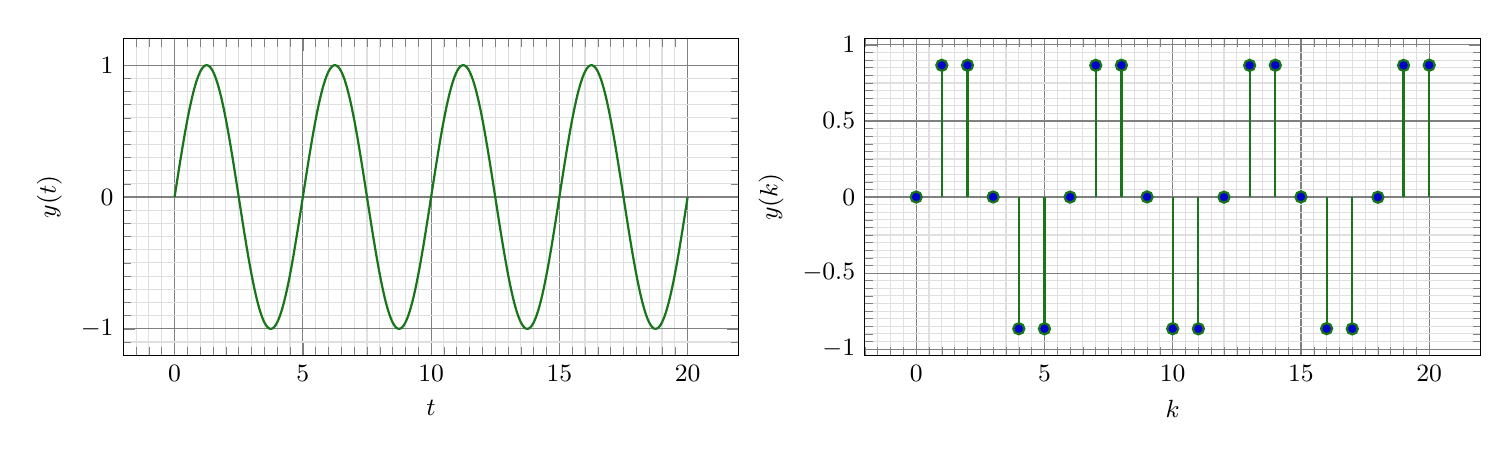
\begin{tikzpicture}
\begin{groupplot}[
  group style={group size=2 by 2, horizontal sep=16mm, vertical sep = 16mm},
  height=5.6cm,width=9.4cm,
  /tikz/font=\small,
  %xtick={1},
  %ytick=\empty,
  %xlabel={$t$ [s]},
  %ylabel={$y(t),\, u(t)$},
  %xmin=-\axlim,
  %xmax=6,
  %ymin=-0.2,
  %ymax=1.3,
  %axis lines=middle,
  grid = both,
  minor tick num=9,
  minor grid style={gray!25},
  major grid style={black!50},
  clip=false,
  ]

  \pgfmathsetmacro{\omegan}{pi*0.4}
  \pgfmathsetmacro{\myh}{pi/3/\omegan}

  \nextgroupplot[ylabel={$y(t)$}, xlabel={$t$},]
  \addplot+[black!60!green!90, thick, no marks, domain=0:20, samples=400] { sin(deg(\omegan*x))};


  \nextgroupplot[ylabel={$y(k)$}, xlabel={$k$},]
  \addplot+[black!60!green!90, thick, ycomb, domain=0:20, samples=21] { sin(deg(\omegan* \myh * x))}; 
  \end{groupplot}


\end{tikzpicture}
\end{document}

